\documentclass[11pt,a4paper]{article}

% Packages
\usepackage[utf8]{inputenc}
\usepackage[T1]{fontenc}
\usepackage{amsmath,amssymb}
\usepackage{graphicx}
\usepackage{hyperref}
\usepackage{booktabs}
\usepackage{xcolor}
\usepackage[margin=1in]{geometry}
\usepackage{natbib}
\usepackage{tikz}
\usetikzlibrary{arrows.meta, positioning, shapes.geometric}

\hypersetup{
    colorlinks=true,
    linkcolor=blue,
    citecolor=blue,
    urlcolor=blue
}
\setlength{\emergencystretch}{3em}

\title{Cognitive Memory for AI Agents:\\Decay Floors, Emergent Core Memories, and Retrieval-Driven Reinforcement}

\author{
  Bhekani Khumalo\\
  Independent Researcher\\
  \texttt{hello@bhekani.com}\\
  \url{https://github.com/planetaryescape/blah.chat}
}

\date{May 2026}

\begin{document}

\maketitle

\begin{abstract}
Most AI memory systems innovate at the edges of the memory lifecycle: deciding what to extract and how to retrieve it. The middle---what happens to a memory after it is stored and before it is retrieved---remains comparatively underexplored. Memories persist at the same weight they had on day one, whether they are an hour old or a month old, accessed fifty times or never. This paper presents \texttt{cognitive-memory}, an open-source memory architecture for LLM-based agents that draws on cognitive science to address this gap. We\footnote{This paper uses the editorial ``we'' throughout, following common convention in computer science. The work is solely that of the listed author.} introduce six design contributions: (1)~\emph{decay floors}, where memories fade according to Ebbinghaus-inspired exponential decay but never reach zero, preserving the possibility of future reactivation; (2)~\emph{emergent core memory detection}, where memories earn protected status through repeated access and cross-session stability rather than only through explicit tagging; (3)~\emph{two-tier retrieval boosting}, where direct retrieval and associative co-retrieval produce different reinforcement magnitudes, modelling the distinction between active recall and passive priming; (4)~\emph{associative memory linking} with differential reinforcement, where co-retrieved memories form and strengthen bidirectional connections; (5)~\emph{tiered hot/cold storage} inspired by the Complementary Learning Systems framework and Tulving's availability--accessibility distinction, where faint memories migrate out of the vector index but remain recoverable through associative retrieval or explicit deep recall; and (6)~\emph{reversible consolidation}, where superseded originals are preserved in cold storage rather than deleted, accessible as associated children of their summaries or via a deep recall retrieval mode analogous to the reactivation of silent engrams. We situate these mechanisms within the broader landscape of agent memory research, contrast our design philosophy with recent work such as FadeMem, describe a production deployment backing a consumer chat application, and report an empirical evaluation on LoCoMo and LongMemEval-S along with a controlled long-term-interaction benchmark. On LoCoMo we recover an overall F1 of 44.8\% with multi-hop F1 of 48.5\%; on LongMemEval-S we reach 70.2\% task-averaged accuracy, competitive with ENGRAM-class single-stage memory systems; ablations indicate that power-law decay is the single largest contributor; and on the controlled benchmark we retain 100\% of identity-critical facts across a 30-day mixed-access window.
\end{abstract}

\section{Introduction}

Large language models are stateless. Every inference is a fresh start. To build agents that maintain continuity across sessions, developers must bolt on external memory systems---and a growing ecosystem of tools exists to do exactly that \citep{chhikara2024mem0, packer2023memgpt, sumers2024coala}. These systems have gotten quite good at two things: extracting salient information from conversations, and retrieving relevant memories when prompted. But between extraction and retrieval lies a dead zone. Once stored, memories sit in a database with the same weight and accessibility they had on the day they were created.

This is not how biological memory works. Human memory is dynamic: it strengthens with use, weakens with neglect, and selectively preserves information that has proven important over time \citep{ebbinghaus1885, bjork1992new}. Crucially, forgetting is not a failure mode but an adaptive feature. Richards and Frankland~\citeyearpar{richards2017persistence} argue that the goal of memory is not faithful information transmission but rather guiding intelligent decision-making in noisy, changing environments. Partial forgetting enables generalization by stripping away context-specific details and preserving underlying patterns.

For AI agents, the engineering consequences of ignoring this middle phase are concrete. A memory system that retains everything at full strength produces context windows bloated with noise, stale facts weighted equally to fresh ones, and no way to distinguish a recurring preference from a passing remark. Consolidation---compressing old memories into summaries---is the field's most common response, but it is lossy and irreversible: the original memories are destroyed, and with them the ability to recover details that may become relevant again.

This paper presents an alternative approach. Our system, \texttt{cognitive-memory}, implements biologically-inspired decay that dims memories without destroying them, retrieval-driven reinforcement that strengthens memories through use, and emergent core memory detection that protects critical information. The key philosophical commitment is that \textbf{a memory should not be pruned merely because it has become hard to retrieve}. Instead, memories fade to a floor: regular memories to a faint but non-zero level, core memories to a high floor that keeps them always accessible. This preserves the possibility of reactivation---the everyday experience of a forgotten detail flooding back when triggered by the right cue.

We contribute: (1) a formal architecture grounded in specific cognitive science mechanisms; (2) several design elements not present in related work, particularly decay floors, emergent core memory promotion, and two-tier retrieval boosting; (3) an open-source implementation available as TypeScript and Python SDKs; (4) a description of its deployment in a production chat application, \texttt{blah.chat};\footnote{\url{https://blah.chat}} and (5) an empirical evaluation on LoCoMo, LongMemEval-S, and a controlled long-term-interaction benchmark targeted at the architectural claims (Section~\ref{sec:evaluation}).

\section{Related Work}

\subsection{Taxonomic Foundations}

The CoALA framework \citep{sumers2024coala} provides the most influential taxonomy for agent memory, distinguishing working memory (short-term, in-context) from long-term memory (episodic, semantic, procedural). CoALA draws on the SOAR cognitive architecture and identifies memory management as a key area for future development, though its focus is primarily on the structural organization of memory rather than temporal dynamics.

\subsection{Memory Architectures for Agents}

Park et al.~\citeyearpar{park2023generative} introduced the generative agents architecture, where agents maintain a ``memory stream'' of observations and synthesize higher-level reflections over time. Their retrieval function combines recency, importance, and relevance---an early recognition that not all memories should be weighted equally. However, the recency signal is a simple time-based decay with no mechanism for retrieval-driven strengthening or differentiated decay rates.

MemGPT \citep{packer2023memgpt} models agent memory on an operating system's virtual memory hierarchy, with a core memory (in-context) and archival memory (out-of-context) layer. The agent manages its own context through explicit read/write operations. This is an architectural innovation in \emph{how} memory is organized, but it does not address the temporal dynamics of what happens to memories over time.

Mem0 \citep{chhikara2024mem0} provides a unified memory layer with extraction, deduplication, and retrieval. Recent versions describe decay mechanisms where ``memories strengthen when recalled and naturally decay over time if unused,'' though the implementation details and decay model are not fully specified in published materials.

\subsection{Forgetting Mechanisms}

The most directly related work is FadeMem \citep{wei2026fademem}, published in January 2026. FadeMem implements Ebbinghaus-inspired exponential decay across a dual-layer (short-term/long-term) memory hierarchy, with retention modulated by semantic relevance, access frequency, and temporal patterns. It incorporates LLM-guided conflict resolution and memory fusion, and demonstrates improvements over Mem0 and MemGPT on multiple benchmarks. Our work shares the same cognitive science inspiration but differs in several design choices detailed in Section~\ref{sec:comparison}.

MemoryBank \citep{zhong2024memorybank} incorporates the Ebbinghaus forgetting curve to model memory strength decay and supports continual memory updating and user profile construction. SAGE \citep{sage2024} combines the Ebbinghaus curve with linguistic knowledge to optimize memory management, applying part-of-speech priority to determine information retention. Memoria \citep{memoria2023} addresses what it calls the ``fateful forgetting problem'' through a human-inspired memory architecture. MemOS \citep{kang2025memos} introduces TTL-based lifespan policies and state transitions (Generated $\rightarrow$ Activated $\rightarrow$ Merged $\rightarrow$ Archived $\rightarrow$ Expired).

\paragraph{Concurrent and post-dating systems.} Three systems published shortly before or during our evaluation window sit close to our problem framing on long-horizon conversational memory benchmarks. ENGRAM \citep{patel2025engram} routes turns into episodic, semantic, and procedural records and reports state-of-the-art accuracy on LongMemEval-S at the time it was posted; it is the strongest single-stage baseline against which we compare. TiMem \citep{li2026timem} organises conversations through a Temporal Memory Tree that consolidates raw observations into progressively abstracted persona representations and reports 76.88\% on LongMemEval-S, exceeding ENGRAM and our own 70.2\%. EverMemOS \citep{hu2026evermemos} implements an engram-inspired lifecycle (episodic trace formation, semantic consolidation, reconstructive recollection) and reports 83.0\% on LongMemEval. Both TiMem and EverMemOS post-date our evaluation runs but pre-date publication of this paper; we acknowledge them here so that our LongMemEval-S result is not over-claimed (it is competitive with ENGRAM-class single-stage systems, but is not state-of-the-art on this benchmark as of mid-2026). Our contribution is an architectural one---decay floors, emergent core promotion, two-tier boosting---rather than a benchmark-leading numerical one, and the empirical results in Section~\ref{sec:evaluation} are reported as evidence that the architecture behaves as designed at competitive performance levels, not as a leaderboard claim.

The ``Memory in the Age of AI Agents'' survey \citep{liu2025memory} provides the most comprehensive recent overview, categorizing forgetting as one of three branches of memory evolution alongside consolidation and updating. That survey's taxonomy distinguishes memory by \emph{form} (token-level, parametric, latent) and \emph{function} (factual, experiential, working). Our system operates entirely at the token level---memories are discrete text records in an external store---and primarily serves the factual memory function, maintaining persistent knowledge about users and their preferences across sessions. This confirms that forgetting is an active area of research, though one still in its early stages with no dominant approach.

\subsection{Cognitive Science Foundations}

Our architecture draws on several established results from cognitive science and neuroscience:

\begin{itemize}
    \item \textbf{Ebbinghaus forgetting curves} \citep{ebbinghaus1885, murre2015replication}: Memory retention follows exponential decay, with the steepest drop occurring shortly after encoding.
    \item \textbf{Spaced repetition effects} \citep{cepeda2006distributed}: Memories accessed at increasing intervals develop greater long-term stability than those accessed in massed practice.
    \item \textbf{Spreading activation} \citep{collins1975spreading}: Retrieving one memory activates semantically related memories, with activation strength decreasing with associative distance.
    \item \textbf{Synaptic tagging} \citep{frey1997synaptic}: Certain memories receive biochemical tags during encoding that mark them for preferential long-term consolidation, independent of subsequent access patterns.
    \item \textbf{Adaptive forgetting} \citep{richards2017persistence}: The interaction between persistence and transience optimizes memory-guided decision-making. The goal of memory is not accurate recording but flexible behaviour in changing environments.
    \item \textbf{Intentional forgetting} \citep{popov2019forgetting}: Forgetting can be an effortful, resource-consuming process that actively aids memory for target items. Our system implements only passive decay rather than directed forgetting, but this work motivates the broader view that forgetting is functional rather than merely a failure of retention.
    \item \textbf{Availability vs.\ accessibility} \citep{tulving1966availability}: Apparent forgetting often reflects a failure of retrieval (accessibility) rather than a loss of stored information (availability). Memories may be intact in storage but inaccessible without appropriate cues.
    \item \textbf{Complementary Learning Systems} \citep{mcclelland1995complementary}: The brain maintains two complementary memory stores---a fast-learning, fast-decaying hippocampal system and a slow-learning, stable neocortical system---with gradual migration of memories between them.
    \item \textbf{Silent engrams} \citep{ryan2022forgetting}: Forgotten memories may persist as engram ensembles that are available but inaccessible through natural retrieval cues, recoverable only through artificial stimulation. This suggests that much natural forgetting is a state change in accessibility rather than erasure.
\end{itemize}

\section{Architecture}

The \texttt{cognitive-memory} system operates as a middleware layer between an LLM-based agent and its vector store. When the agent produces or encounters information worth remembering, the system extracts structured memory objects, assigns initial parameters, stores them with embeddings, and manages their lifecycle over time. On retrieval, the system queries semantically, applies retention-weighted scoring, boosts accessed memories, and returns results ordered by composite relevance.

\subsection{Memory Representation}

Each memory is represented as a structured object with the following fields:

\begin{table}[h]
\centering
\small
\begin{tabular}{@{}lll@{}}
\toprule
\textbf{Field} & \textbf{Type} & \textbf{Description} \\
\midrule
\texttt{content} & string & Natural language content \\
\texttt{category} & enum & \texttt{episodic}, \texttt{semantic}, \texttt{procedural}, \texttt{core} \\
\texttt{importance} & float [0,1] & LLM-assessed salience at extraction \\
\texttt{stability} & float [0,1] & Resistance to decay; increases with use \\
\texttt{accessCount} & int & Number of times retrieved \\
\texttt{lastAccessedAt} & datetime & Timestamp of most recent retrieval \\
\texttt{createdAt} & datetime & Timestamp of creation \\
\texttt{associations} & list & Links to related memories with weights \\
\bottomrule
\end{tabular}
\caption{Memory object schema. The \texttt{core} category triggers elevated decay floors and is assigned either by LLM classification at extraction or by emergent promotion (Section~\ref{sec:core}).}
\label{tab:schema}
\end{table}

\subsection{Decay Model}
\label{sec:decay}

Retention is computed as a modified exponential decay function:

\begin{equation}
R(m) = \max\left(f_m,\; \exp\!\left(\frac{-\Delta t(m)}{S(m) \cdot B(m) \cdot \tau_c}\right)\right)
\label{eq:retention}
\end{equation}

\noindent where:
\begin{itemize}
    \item $R(m) \in [f_m, 1]$ is the retention score for memory $m$
    \item $f_m$ is the \emph{decay floor} (see Section~\ref{sec:floors})
    \item $\Delta t(m)$ is days since last access
    \item $S(m) \in [0, 1]$ is the stability parameter, representing resistance to decay
    \item $B(m) = 1 + (\text{importance}(m) \times 2)$, capped at 3, is the importance boost
    \item $\tau_c$ is the base retention time constant, dependent on memory category
\end{itemize}

Base retention time constants are differentiated by category to reflect the different temporal profiles of memory types documented in cognitive science \citep{finley2025expanded}:

\begin{table}[h]
\centering
\small
\begin{tabular}{@{}lrl@{}}
\toprule
\textbf{Category} & \textbf{$\tau_c$ (days)} & \textbf{Rationale} \\
\midrule
Episodic & 30 & Event memories fade relatively quickly \\
Semantic & 90 & Factual knowledge persists longer \\
Procedural & $\infty$ & Skills and procedures do not decay \\
Core & 90 & High floor dominates; base rate matters less \\
\bottomrule
\end{tabular}
\caption{Base retention time constants by memory category. Larger values produce slower forgetting.}
\label{tab:decay}
\end{table}

\subsection{Decay Floors: Never Delete}
\label{sec:floors}

The central design commitment of this architecture is that \textbf{no memory reaches zero}. The decay floor $f_m$ enforces a minimum retention score:

\begin{equation}
f_m = \begin{cases}
0.60 & \text{if } \texttt{category}(m) = \texttt{core} \\
0.02 & \text{otherwise}
\end{cases}
\end{equation}

A regular memory at its floor (2\% retention) is unlikely to surface in normal retrieval, but it is not annihilated by the scoring function. Retrieval uses a softened accessibility term, $R^\alpha$ with default $\alpha=0.3$, so a floor-retained memory has $0.02^{0.3} \approx 0.309$ accessibility. With a highly specific semantic match of 0.9, its final score is therefore approximately $0.9 \times 0.309 \approx 0.278$, rather than $0.018$ under linear retention weighting. We term memories below 15\% retention \emph{faint}---rarely surfaced, but not pruned by decay alone.

This stands in deliberate contrast to systems that prune memories below a threshold. FadeMem, for instance, imposes hard capacity caps (1000 long-term memories, 500 short-term) and allows memories to decay to removal \citep{wei2026fademem}. Our position is that deletion can destroy information that may become relevant in unpredictable future contexts. The cost of storing faint text records is usually small; the cost of permanently losing them is hard to predict.

This mirrors the neurobiological reality that memories are rarely truly erased. Rather, they become increasingly difficult to access as retrieval pathways weaken, while the underlying traces persist \citep{wixted2004psychology}. The common experience of a long-forgotten detail returning vividly when triggered by the right cue---a smell, a name, a location---is evidence that the memory was dimmed, not deleted.

To make this concrete: consider a user who mentions their cat's name in session 3, then never references it again. By session 20, that memory has decayed to its 2\% floor. In a deletion-based system, it is gone. In ours, it persists as a faint memory, invisible to normal retrieval. But when the user asks in session 47, ``what was my cat called?''---a query with high semantic similarity to exactly that memory---the retention floor allows it to surface. The retrieval boost then begins restoring its stability, and the memory re-enters active circulation. This is the specific behaviour that decay floors are designed to preserve, and it is not recoverable once a memory has been pruned.

\subsection{Core Memory Detection}
\label{sec:core}

Core memories are those that should remain highly accessible regardless of access patterns: a user's name, critical allergies, fundamental preferences. We implement two complementary pathways to core status. The first is loosely analogous to synaptic tagging \citep{frey1997synaptic}, in that certain memories receive preferential treatment at encoding time, though our mechanism (LLM classification) is far simpler than the biological process. The second pathway mirrors use-dependent consolidation:

\paragraph{Explicit tagging.} At extraction time, the LLM classifies whether a memory represents identity-critical information (names, medical conditions, family relationships). If so, it is immediately assigned \texttt{category = core} with the 60\% floor.

\paragraph{Emergent promotion.} Memories that were not initially tagged as core can earn core status through sustained use. A memory is promoted to core when it meets three criteria simultaneously:

\begin{enumerate}
    \item \textbf{High access count}: retrieved more than a configurable threshold number of times (default: 10)
    \item \textbf{High stability}: the stability parameter exceeds a threshold (default: 0.85)
    \item \textbf{Cross-session persistence}: the memory has been accessed across at least 3 distinct sessions
\end{enumerate}

This emergent pathway reflects the cognitive science observation that core memories in humans are not all tagged at encoding. Many become central to identity through repeated retrieval and emotional reinforcement over time \citep{bjork1992new}. A user's preference for a particular communication style might not seem identity-critical when first expressed, but after being accessed in dozens of conversations, it has functionally become core knowledge about that user.

\subsection{Retrieval Scoring}

When the agent queries memory, results are scored by the product of semantic relevance and a power-law accessibility transform of retention:

\begin{equation}
\text{score}(m, q) = \text{sim}(m, q) \times R(m)^\alpha
\label{eq:score}
\end{equation}

\noindent where $\text{sim}(m, q)$ is the cosine similarity between the memory embedding and the query embedding, $R(m)$ is the retention score from Equation~\ref{eq:retention}, and $\alpha$ controls how aggressively retention suppresses retrieval (default: $\alpha=0.3$). This means two memories with identical semantic content can produce different retrieval scores based on their temporal profiles, while faint memories remain accessible to highly specific cues.

This multiplicative interaction is the mechanism by which the system implements what Richards and Frankland~\citeyearpar{richards2017persistence} describe as memory's role in guiding intelligent decisions: recent, repeatedly-accessed information is foregrounded, while stale or rarely-used information recedes without being eliminated.

\subsection{Two-Tier Retrieval Boosting}
\label{sec:boost}

When a memory is retrieved, its temporal parameters are updated to reflect the access event. We distinguish two tiers of retrieval, inspired by the cognitive distinction between active recall and passive priming via spreading activation \citep{collins1975spreading}:

\paragraph{Direct retrieval.} When a memory is returned as a primary result for a query, it receives a full boost:
\begin{align}
\text{accessCount}(m) &\leftarrow \text{accessCount}(m) + 1 \\
\text{stability}(m) &\leftarrow \min\!\left(1.0,\; \text{stability}(m) + 0.1 \times \min\!\left(2.0,\; \frac{\Delta t(m)}{7}\right)\right)
\end{align}

The stability update implements a spaced repetition effect: memories accessed after a longer gap receive a larger stability increment (up to a cap at 14 days), while memories accessed in rapid succession gain less stability per access \citep{cepeda2006distributed}. Stability is clamped to $[0, 1]$, so a memory that has been frequently accessed over a long period saturates at $S(m) = 1.0$, representing maximum resistance to decay. Figure~\ref{fig:boosting} illustrates the divergence: two memories with identical starting conditions, both retrieved every 7 days, develop markedly different stability and retention profiles depending on whether retrieval is direct or associative. Critically, only the directly retrieved memory accumulates enough stability to cross the core promotion threshold, gaining permanent floor protection that the associatively retrieved memory never earns.

\paragraph{Associative retrieval.} When a memory is not a direct match but is \emph{associated} with a directly retrieved memory (see Section~\ref{sec:associations}), it receives a smaller boost:
\begin{align}
\text{accessCount}(m) &\leftarrow \text{accessCount}(m) + 1 \\
\text{stability}(m) &\leftarrow \min\!\left(1.0,\; \text{stability}(m) + 0.03 \times \min\!\left(2.0,\; \frac{\Delta t(m)}{7}\right)\right)
\end{align}

This two-tier structure captures the observation that being directly recalled strengthens a memory more than being passively activated through association, while still acknowledging that any activation at all has a reinforcing effect.

\begin{figure}[t]
\centering
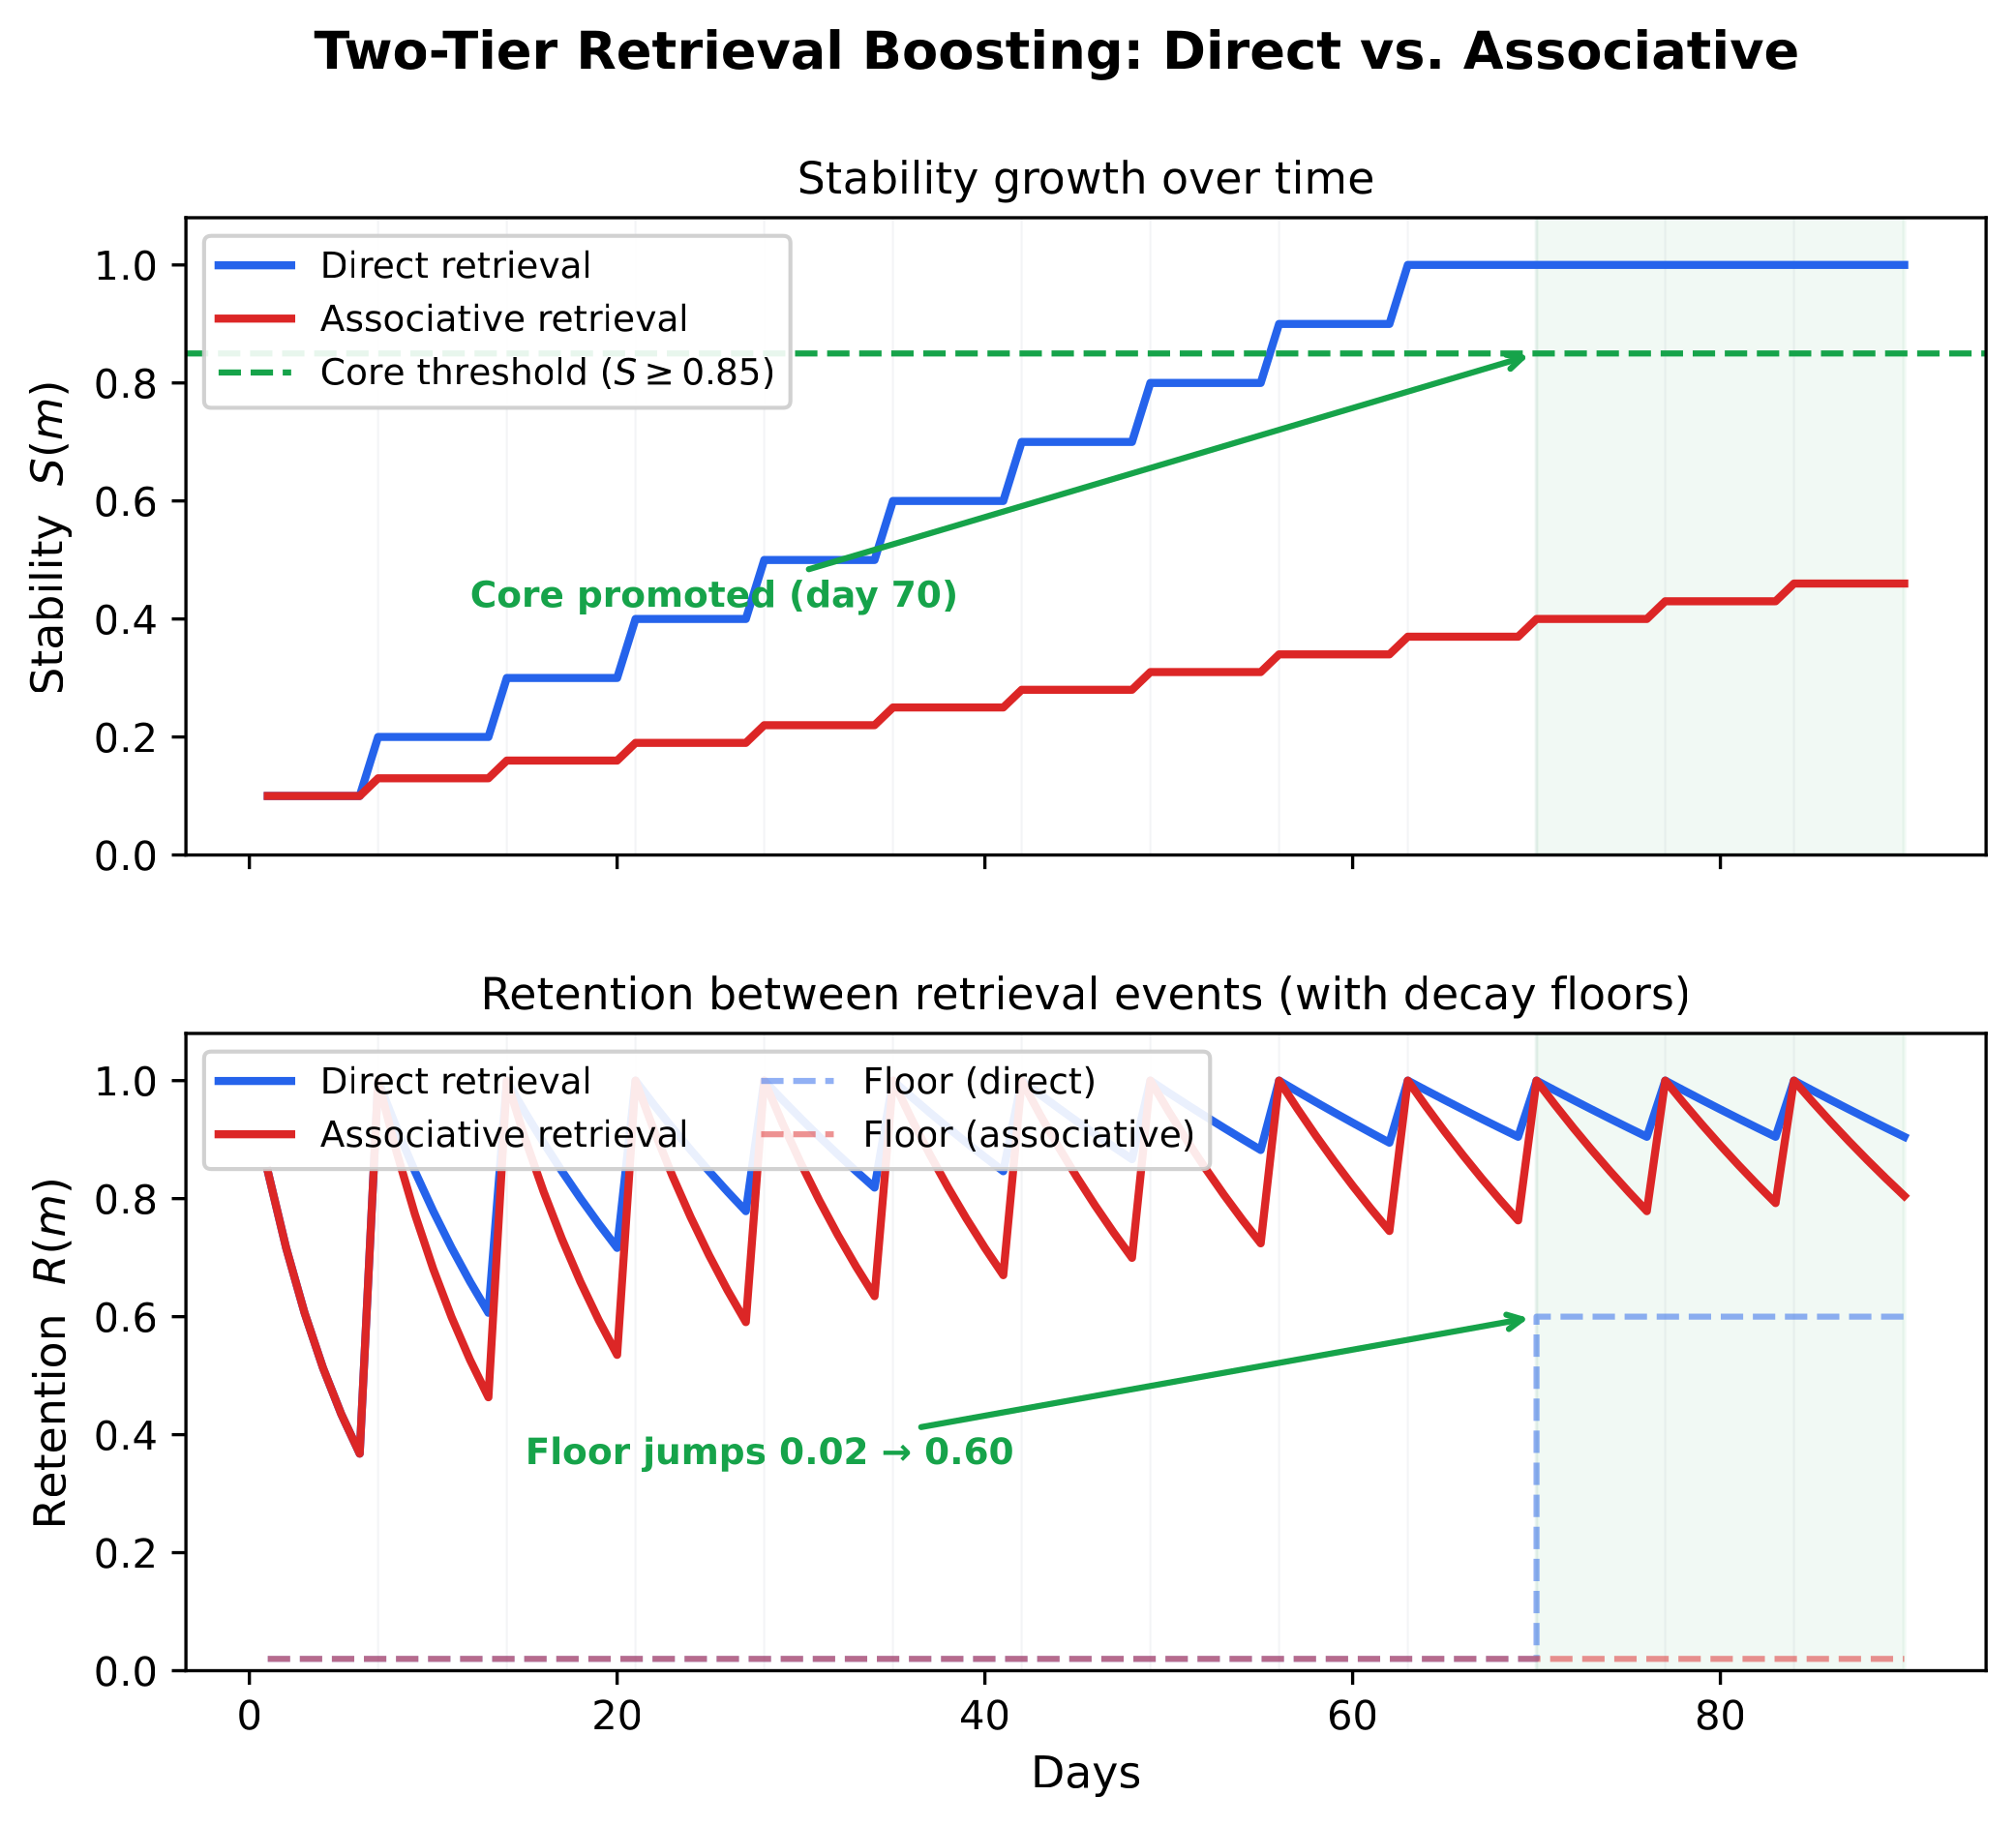
\includegraphics[width=\columnwidth]{boosting_divergence.png}
\caption{Simulated divergence between direct and associative retrieval over 90 days. Both memories start with identical parameters ($S = 0.1$, importance $= 0.5$, episodic category) and are retrieved every 7 days, with new sessions every 14 days. \textbf{Top:} Stability growth. The directly retrieved memory crosses the core promotion threshold ($S \geq 0.85$) at day 70 (green shaded region), while the associatively retrieved memory reaches only $S = 0.46$ and never qualifies. \textbf{Bottom:} Retention between retrieval events. At day 70, the directly retrieved memory's decay floor jumps from 0.02 to 0.60 upon core promotion (blue dashed line), guaranteeing it can never fade below 60\% retention. The associatively retrieved memory's floor remains at 0.02 throughout. The same 12 retrieval events, differentiated only by boost magnitude, produce fundamentally different long-term outcomes: one memory earns permanent protection, the other does not.}
\label{fig:boosting}
\end{figure}

To test whether this divergence is robust to realistic variation in access patterns, we conducted a Monte Carlo analysis with 500 simulation runs. In each run, both memories received the same randomised retrieval schedule: approximately 12 retrieval events (Poisson-distributed) placed at random days within the 90-day window, with new sessions every 14 days. All other parameters were identical to the deterministic case.

The results (Figure~\ref{fig:monte_carlo}) confirm that the divergence is structural rather than an artefact of regular scheduling. Directly retrieved memories achieved core promotion in 76.8\% of runs (384/500), with a median promotion day of 68 (IQR: 60--76). Associatively retrieved memories achieved core promotion in 0\% of runs. At day 90, directly retrieved memories had mean stability $0.985 \pm 0.052$, while associatively retrieved memories reached only $0.417 \pm 0.044$. The confidence bands in Figure~\ref{fig:monte_carlo} show that even the 10th-percentile direct retrieval trajectory exceeds the 90th-percentile associative trajectory by approximately day 40. This separation is a consequence of the 3.3$\times$ boost ratio (0.1 vs.\ 0.03) compounding over repeated access events; it is not sensitive to the specific scheduling of those events.

\begin{figure}[t]
\centering
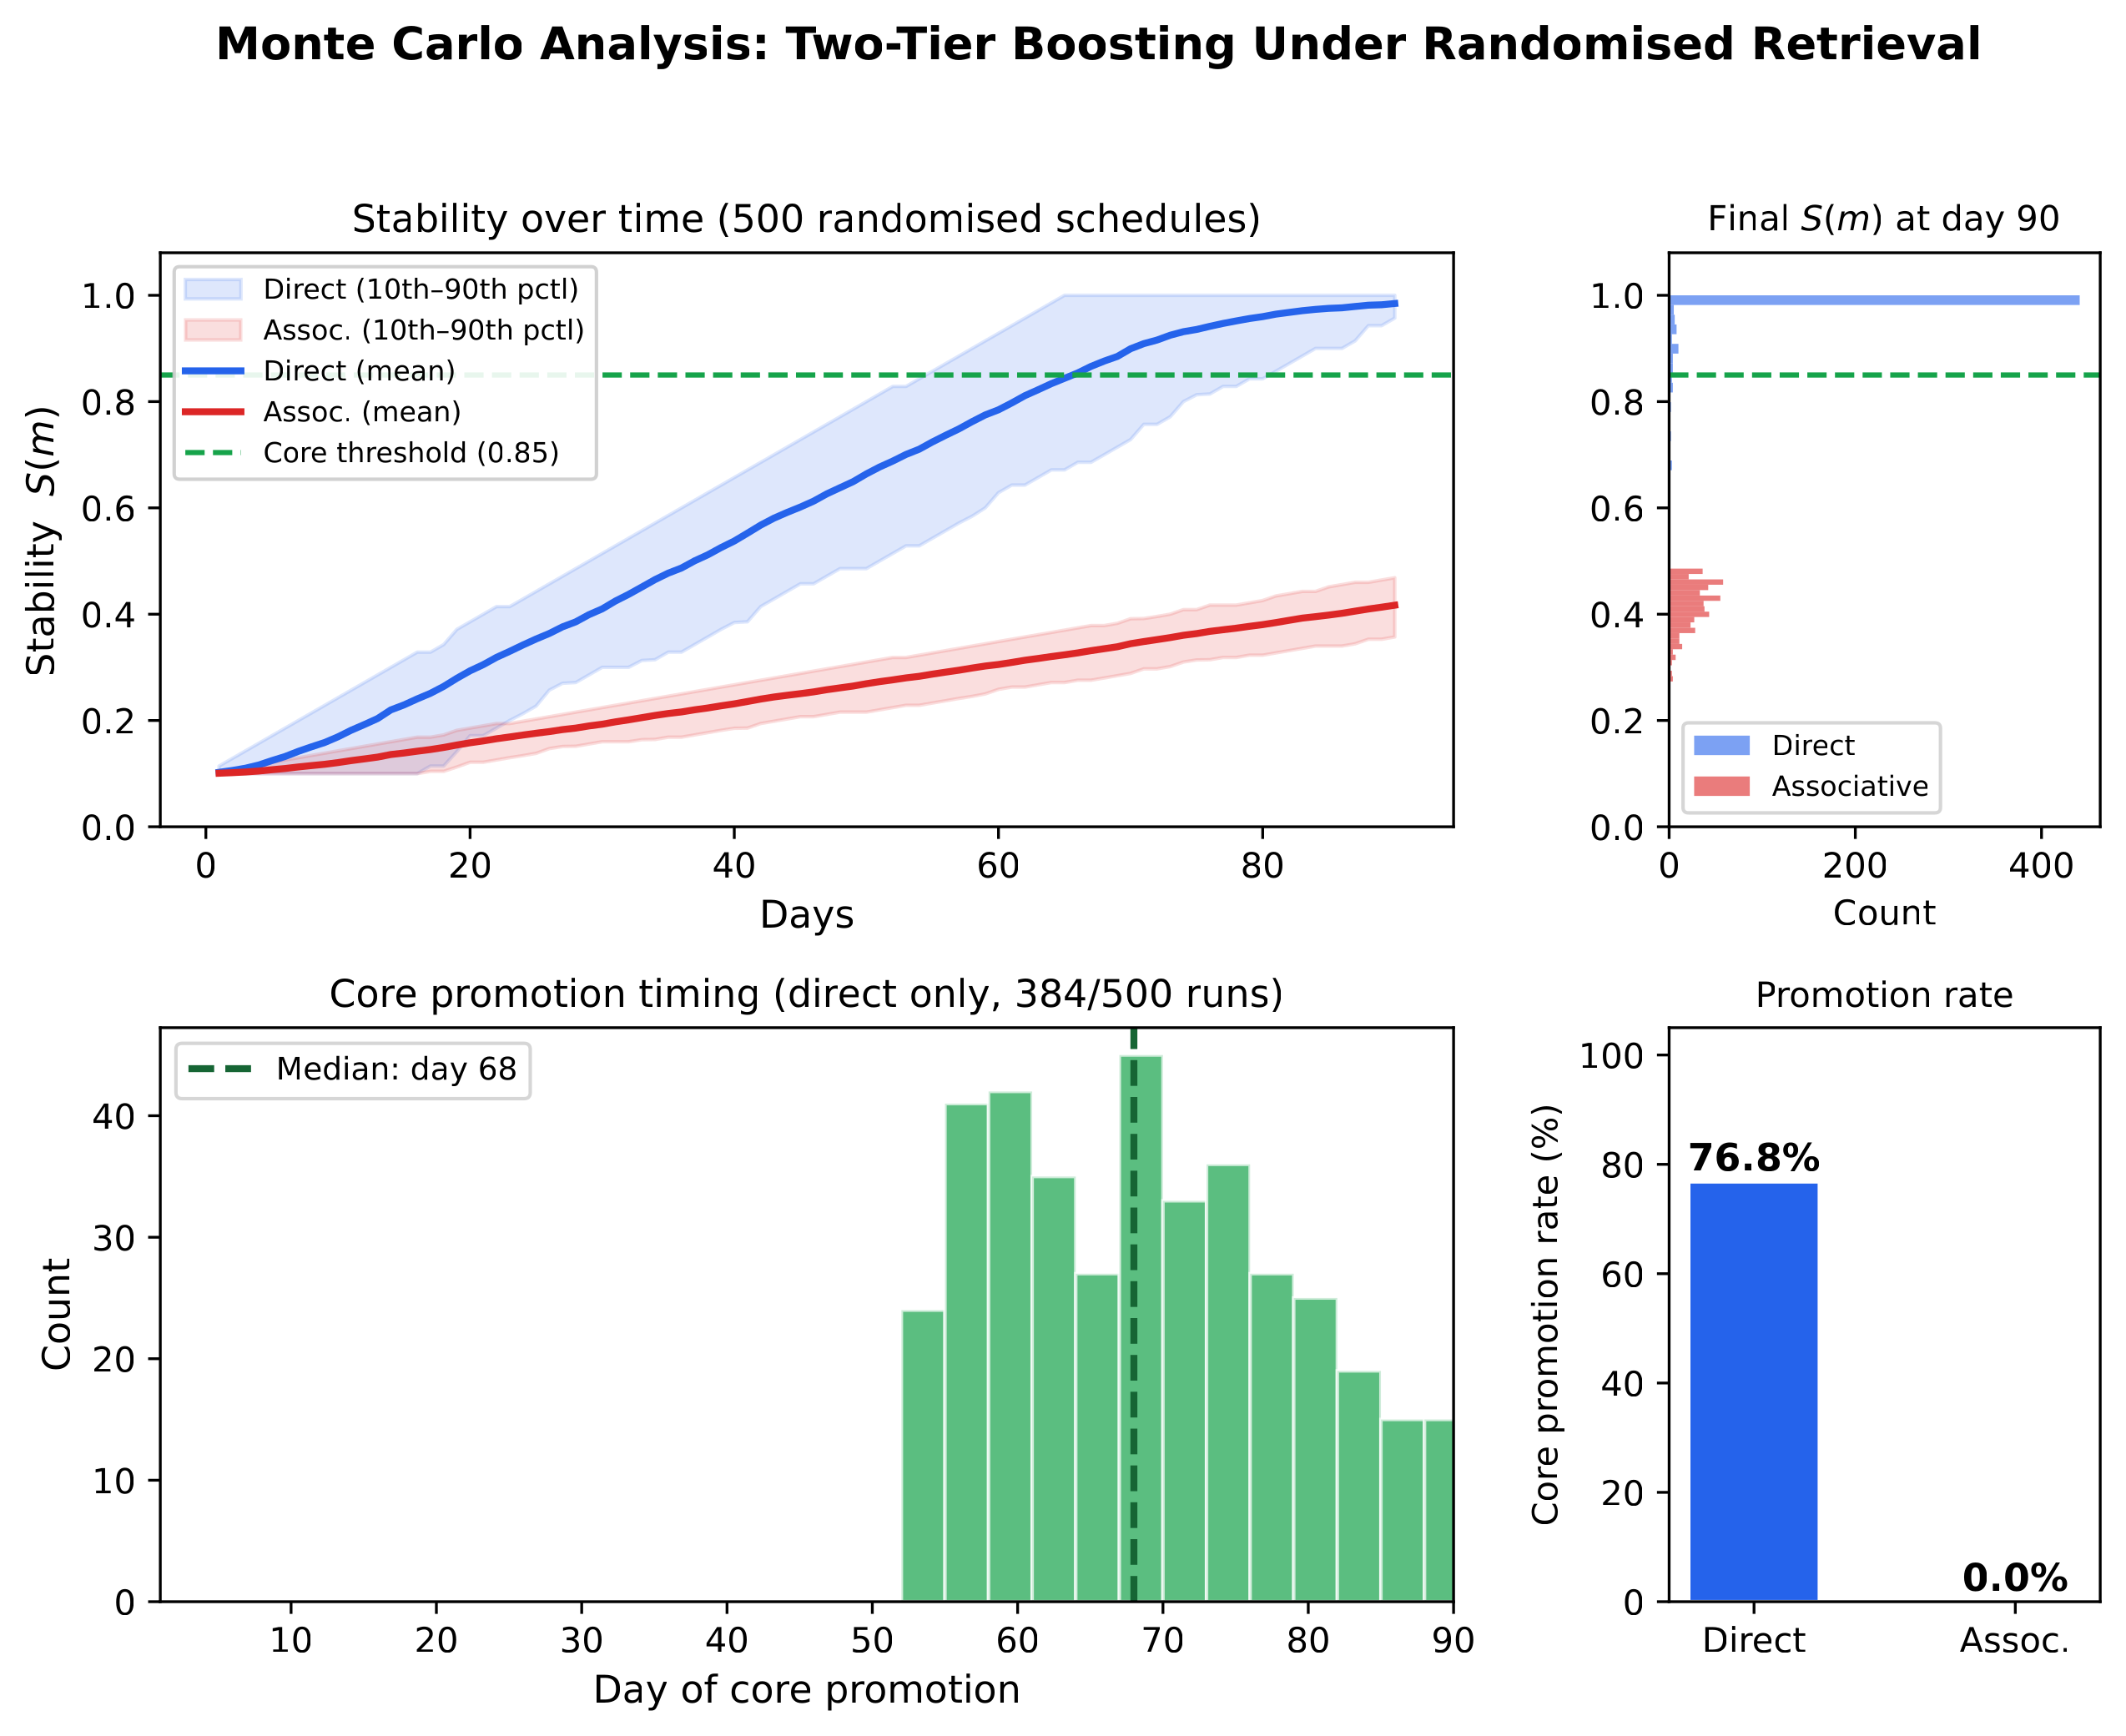
\includegraphics[width=\columnwidth]{monte_carlo.png}
\caption{Monte Carlo analysis of two-tier boosting across 500 randomised retrieval schedules ($\sim$12 Poisson-distributed events per run, sessions every 14 days). \textbf{Top left:} Mean stability trajectories with 10th--90th percentile bands. The direct retrieval mean crosses the core threshold around day 60; the associative mean never approaches it. \textbf{Top right:} Distribution of final stability at day 90, showing near-complete separation between the two tiers. \textbf{Bottom left:} Distribution of core promotion timing for direct retrieval (median: day 68). \textbf{Bottom right:} Core promotion rates: 76.8\% for direct, 0\% for associative.}
\label{fig:monte_carlo}
\end{figure}

\subsection{Associative Memory Graph}
\label{sec:associations}

Memories form bidirectional associations when they are retrieved together or created in the same context. Each association has a weight $w \in [0, 1]$ that strengthens with co-retrieval:

\begin{equation}
w(a, b) \leftarrow \min(1.0,\; w(a, b) + 0.1)
\end{equation}

When memory $a$ is directly retrieved, the system checks its associations and returns any associated memory $b$ where $w(a, b)$ exceeds a threshold (default: 0.3), provided $b$'s own retention score is above a minimum. Associated memories are marked as such in the results and receive the smaller associative boost described above.

This mechanism models spreading activation \citep{collins1975spreading}: retrieving a concept activates related concepts, with activation strength proportional to association weight. Over time, frequently co-retrieved memories develop strong bidirectional links, while associations between rarely co-accessed memories weaken. Specifically, association weights decay exponentially based on time since last co-retrieval:

\begin{equation}
w(a, b) \leftarrow w(a, b) \times \exp\!\left(\frac{-\Delta t_w}{90}\right)
\end{equation}

\noindent where $\Delta t_w$ is days since the association was last strengthened (i.e., since $a$ and $b$ were last co-retrieved). The 90-day time constant means unused associations fade slowly but steadily: after 90 days without co-retrieval, an association retains approximately 37\% of its weight; after 180 days, approximately 13\%. Associations that fall below the retrieval threshold (0.3) no longer trigger associative retrieval, though they are not deleted and can be restored if co-retrieval resumes.

\subsection{Consolidation}
\label{sec:consolidation}

The system includes a consolidation process that clusters fading memories (retention below 0.2) by semantic similarity and compresses groups of five or more into summary memories. However, unlike typical consolidation approaches that discard originals after compression, our revised policy preserves them through the tiered storage mechanism described below. Original memories are clamped to the regular floor (0.02), marked with metadata linking them to their superseding summary (\texttt{supersededBy=<summaryId>}), and migrated to cold storage. In normal retrieval, superseded originals are not eligible as direct hits. They surface only as associated children when their superseding summary is retrieved, providing a lossless path back to the raw details when needed.

\subsection{Tiered Storage}
\label{sec:tiered}

A fundamental tension exists in any memory system that avoids pruning by decay alone: the stored corpus grows monotonically. While individual text records are cheap to store, vector similarity search degrades as the candidate pool expands. We address this with a two-tier architecture inspired by the neuroscientific distinction between memory \emph{availability} and \emph{accessibility} \citep{tulving1966availability}.

Tulving and Pearlstone's foundational finding demonstrated that memories can be intact in storage (available) yet fail to be retrieved (inaccessible) without appropriate cues. Recent neuroscience has reinforced this view: engrams corresponding to apparently forgotten memories persist in ``silent'' states that resist natural reactivation but can be recovered through artificial stimulation \citep{ryan2022forgetting, guskjolen2024forgetting}. At the systems level, the Complementary Learning Systems framework \citep{mcclelland1995complementary} posits a fast-learning, fast-decaying hippocampal store that gradually transfers memories to a slower, more stable neocortical store---a two-tier architecture with migration driven by time and consolidation.

Our tiered storage implements a computational analogue. The \textbf{hot store} is a vector-indexed table supporting embedding similarity search: this is the agent's working memory, containing all active, recently accessed, and core memories. The \textbf{cold store} is a plain key-value table in the same database---no embeddings indexed, no similarity search, accessed only by ID. Memories migrate from hot to cold when their retention has remained at floor for a configurable threshold (default: 7 consecutive days with zero retrievals). Core memories are exempt from migration. Superseded originals from consolidation are migrated to cold storage immediately.

The cold store is not a graveyard. When a hot memory is retrieved and has associations pointing to cold IDs, the system performs an O(1) lookup by identifier and applies associative scoring. If a cold memory surfaces through this path and receives a retrieval boost, it is migrated back to the hot store---re-indexed for similarity search and fully reactivated. This bidirectional migration mirrors the concept of silent engrams: memories that are available but not accessible through normal retrieval, yet recoverable when the right associative cue provides a path back. Deployments can additionally configure a long cold-storage TTL (default: 180 days), after which a cold record is converted into a lightweight archival stub; stubs remain excluded even in deep recall. The benchmark results reported below operate within horizons shorter than this TTL.

\paragraph{Deep recall mode.} In neuroscience, ``silent engrams'' are memory traces that persist biologically but cannot be reactivated through natural retrieval cues; they require artificial stimulation (e.g., optogenetic activation of dentate gyrus neurons) to produce memory expression \citep{ryan2022forgetting, guskjolen2024forgetting}. Our superseded originals in cold storage are computationally analogous: they exist, they are available in Tulving's sense, but they are inaccessible through normal similarity search because they have been removed from the vector index.

Deep recall mode provides the artificial stimulation. Normal search excludes cold memories, superseded originals, and lightweight stubs. The system exposes an optional retrieval parameter (\texttt{deep\_recall: true}) that temporarily includes cold memories and superseded originals in the direct candidate set, while stubs remain excluded. Superseded and expired items receive a multiplicative penalty (default: $0.5\times$ their normal score) to ensure they surface only when the query strongly matches. This is implemented as a parameter on the canonical \texttt{search()} function rather than a system-wide mode, keeping the API stateless and allowing the calling agent (or user) to decide when exhaustive recall is warranted---for example, when the user asks ``what exactly did I say about X three months ago?'' and a consolidated summary is insufficient. The compatibility \texttt{retrieve()} API delegates to \texttt{search()} and maps results back to the older scored-memory shape.

This design reflects the broader principle from Tulving and Pearlstone's work that apparent forgetting often represents a retrieval problem, not a storage problem \citep{tulving1966availability}. By changing the retrieval conditions (expanding the candidate set), information that was functionally forgotten becomes accessible again---without requiring that it pollute normal retrieval at all other times.

\paragraph{Scaling behaviour.} To evaluate whether tiered storage bounds the hot index across realistic usage patterns, we simulated one year of operation under six scenarios varying the memory ingestion rate (2--10 memories/day), query frequency (1--12 queries/day), and results per query (3--4). Figure~\ref{fig:cold_storage} shows the results. Across all scenarios, the hot index stabilises at 7--11\% of total memories by day 365. In the moderate case (4 memories/day, 3 queries/day), the hot index settles at 124 entries (7.0\% of 1,774 total). Even in the most challenging scenario---bursty ingestion at 10 memories/day with only 2 queries/day---the hot index reaches 394 (8.7\% of 4,529 total) and plateaus. The consistency of this range across diverse access patterns suggests that the bounded hot index is a structural property of the architecture rather than an artefact of any particular usage profile.

\begin{figure}[t]
\centering
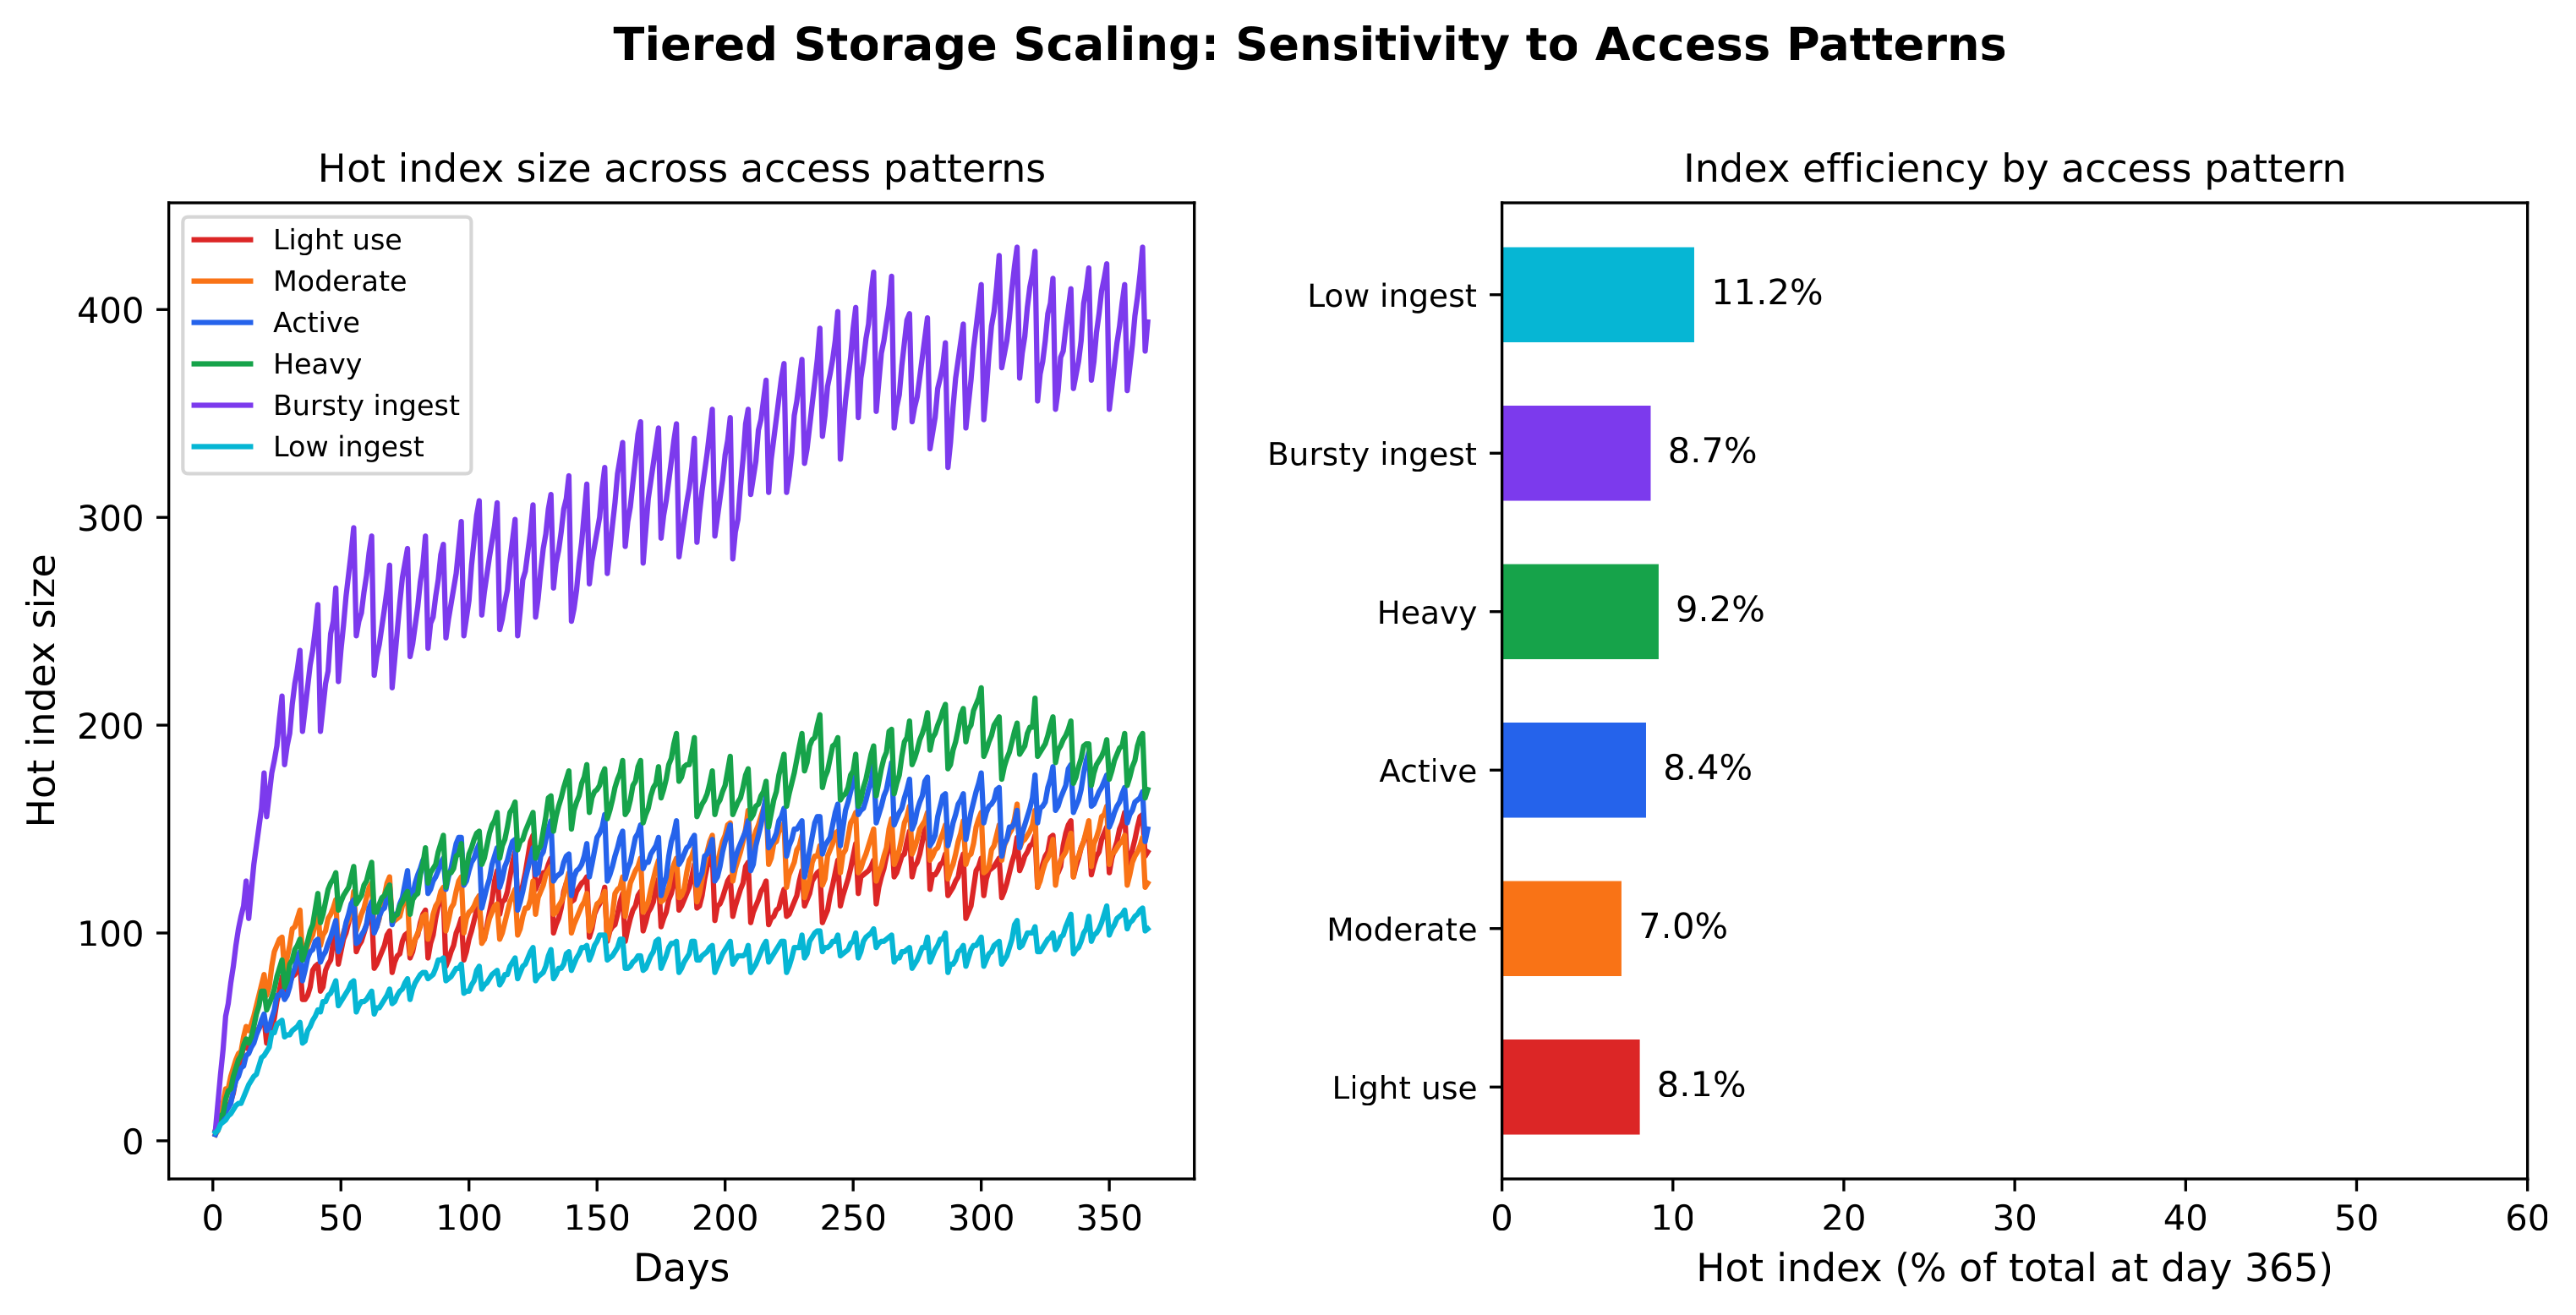
\includegraphics[width=\columnwidth]{cold_storage.png}
\caption{Tiered storage scaling across six access patterns over one simulated year. \textbf{Left:} Hot index size over time. All scenarios plateau; absolute size scales with ingestion rate but growth converges to zero. The bursty ingest scenario (10 memories/day, 2 queries/day) shows the most variance but still stabilises. \textbf{Right:} Hot index as percentage of total memories at day 365. All scenarios converge to the 7--11\% range, indicating that bounded hot index size is robust to access pattern variation.}
\label{fig:cold_storage}
\end{figure}

\paragraph{Caveats.} The preservation-first assumption underlying this architecture is debatable; we discuss the counterevidence from intrinsic forgetting research in Section~\ref{sec:limitations}.

\section{Design Comparison with FadeMem}
\label{sec:comparison}

FadeMem \citep{wei2026fademem} is the most closely related system, sharing our Ebbinghaus-inspired foundation. Table~\ref{tab:comparison} summarises the key differences.

\begin{table}[h]
\centering
\small
\begin{tabular}{@{}p{3cm}p{5.5cm}p{5.5cm}@{}}
\toprule
\textbf{Design Choice} & \textbf{FadeMem} & \textbf{cognitive-memory (ours)} \\
\midrule
Decay endpoint & Memories can decay to removal; hard capacity caps (1000 LTM, 500 STM) & Decay never sets retention to zero; floors at 2\% (regular) and 60\% (core), with optional cold-storage stub conversion after TTL \\
\addlinespace
Memory hierarchy & Dual-layer (STM/LTM) with promotion criteria & Flat store with category-based decay rates; core as a category, not a layer \\
\addlinespace
Core memory & Not implemented as an explicit category; high-importance memories receive elevated retention through scoring but without guaranteed floor protection & Dual-path: LLM tagging at extraction + emergent promotion through use \\
\addlinespace
Retrieval reinforcement & Access strengthens retention & Two-tier: direct retrieval (+full boost) vs.\ associative drag-along (+partial boost) \\
\addlinespace
Associative linking & Not described as a separate mechanism; memory fusion serves a related consolidation role & Bidirectional weighted associations with co-retrieval strengthening \\
\addlinespace
Index scaling & Hard capacity caps (1000 LTM, 500 STM); excess memories pruned & Tiered hot/cold storage; hot index bounded at $\sim$10\% of total (Figure~\ref{fig:cold_storage}) \\
\addlinespace
Conflict resolution & LLM-guided classification into contradiction, update, overlap & LLM-guided detection adopting FadeMem's taxonomy; contradicted core memories are demoted to regular floor (Section~\ref{sec:limitations}) \\
\addlinespace
Evaluation & Benchmark-based (MSC, LoCoMo, LTI-Bench) & Production deployment plus LoCoMo, LongMemEval-S, and a controlled LTI-Bench (Section~\ref{sec:evaluation}) \\
\bottomrule
\end{tabular}
\caption{Design comparison between FadeMem and \texttt{cognitive-memory}.}
\label{tab:comparison}
\end{table}

The most significant philosophical difference is about deletion. FadeMem treats memory removal as a feature: by pruning irrelevant memories, it reduces storage by 45\% and improves retrieval precision. Our position is that the storage cost of retaining faint memories is often negligible for text-based agent memory (unlike, say, multimedia storage), and the unpredictability of future relevance makes early deletion a risky optimisation. We optimise retrieval precision not by removing faint memories but by down-weighting them through the multiplicative scoring in Equation~\ref{eq:score}, which achieves a similar practical effect without pruning active or cold records during normal retrieval.

FadeMem's strengths relative to our system include its LLM-guided conflict resolution---which our system now adopts in deferred form (Section~\ref{sec:limitations})---and its memory fusion mechanism for consolidating related information.

\section{Implementation}

The architecture is implemented as \texttt{cognitive-memory}, an open-source TypeScript package with a Python SDK wrapper. The system is adapter-based: it defines interfaces for vector storage and embedding providers, with default implementations for common backends.

\subsection{Adapter Pattern}

\begin{verbatim}
interface MemoryStore {
  store(memory: Memory): Promise<void>
  query(embedding: number[], limit: number): Promise<Memory[]>
  update(id: string, fields: Partial<Memory>): Promise<void>
}

interface EmbeddingProvider {
  embed(text: string): Promise<number[]>
}
\end{verbatim}

This allows the core decay, boosting, and association logic to remain independent of the storage backend. The system has been tested with Pinecone, pgvector, and in-memory stores.

\subsection{Production Deployment}

The system is deployed in \texttt{blah.chat}, a consumer chat application where users interact with LLM-based agents across multiple sessions. In this deployment, the memory system:

\begin{itemize}
    \item Extracts memories from each conversation turn using an LLM call
    \item Stores them with initial importance scores and category assignments
    \item Retrieves relevant memories at the start of each agent turn, injecting them into the system prompt
    \item Runs decay recalculation periodically (currently on each retrieval event)
    \item Checks for emergent core memory promotion after each retrieval cycle
\end{itemize}

The system is currently serving real users and includes an append-only audit log that records every state change: retrieval boosts, decay recalculations, association updates, core memory promotions, and consolidation events. Each log entry captures the memory ID, event type, old and new values, and a timestamp. This instrumentation enables post-hoc analysis of individual memory lifecycles and is the basis for the production-data study planned in Section~\ref{sec:future}; the benchmark evaluation in Section~\ref{sec:evaluation} uses the same SDK code path.

\section{Evaluation}
\label{sec:evaluation}

We evaluate \texttt{cognitive-memory} on three benchmarks: LoCoMo \citep{maharana2024locomo} for multi-session conversational QA, LongMemEval-S \citep{wu2024longmemeval} for long-horizon memory tasks across six question categories, and a controlled synthetic long-term-interaction harness (LTI-Bench) targeted at the architectural claims of this paper. We additionally report ablations on individual feature contributions, an oracle ceiling for context, and a judge-reliability check.

\subsection{Setup}
\label{sec:eval-setup}

\paragraph{Models.} Memory extraction and answer generation use \texttt{gpt-4o-mini}. Embeddings use \texttt{text-embedding-3-small}. The LongMemEval-S task judge uses \texttt{gpt-4o-2024-08-06}, matching the benchmark's official setup. The LTI-Bench LLM-as-judge uses the same \texttt{gpt-4o-2024-08-06} judge for consistency.

\paragraph{SDK.} The current-refresh LoCoMo, oracle, derived-analysis, and LTI-Bench runs reported here use \texttt{cognitive-memory} SDK \texttt{v0.3.0} installed from the local source tree after the v6 behavior fixes: \texttt{search()} is the canonical retrieval API, \texttt{retrieve()} is a compatibility wrapper, normal search excludes cold/superseded/stub records, deep recall includes cold and superseded records while still excluding stubs, and retrieval scoring uses $\operatorname{sim}(m,q) R(m)^\alpha$ with default $\alpha=0.3$. The LongMemEval-S result comes from the completed recorded 500-question run in the benchmark log. The benchmark repository records exact command, configuration, timestamp, output path, and SDK/worktree provenance in \texttt{experimentlog.md}.

\paragraph{Hardware.} All runs are on a single machine (Apple Silicon, 128 GB RAM). Throughput is bounded by OpenAI API latency rather than local compute.

\paragraph{Adapter configuration.} Default v6 configuration: exponential decay (with a separate condition for power-law), graph expansion at one hop, rerank enabled with factor three, hybrid lexical+dense search disabled (we ablate this). LoCoMo uses top-$k$ of 60 with dual-perspective ingestion and the Mem0-style answer prompt. LongMemEval-S uses top-$k$ of 20 with deep recall and rerank.

\subsection{LoCoMo}
\label{sec:eval-locomo}

LoCoMo is a multi-session conversational QA benchmark with 10 conversations averaging 300 turns and 9k tokens, evaluated on five question categories: single-hop, multi-hop, temporal, open-domain, and adversarial. We score using token F1 against gold answers, following the benchmark's protocol.

Table~\ref{tab:locomo} reports our headline result against published baselines. We achieve an overall F1 of 44.8\%, with multi-hop F1 of 48.5\%---approximately 1.7$\times$ Mem0's reported multi-hop F1 of 28.4\% on the same benchmark. The multi-hop category is the hardest in LoCoMo, requiring the system to combine evidence from multiple sessions; this is also the category where decay-floor and emergent-core mechanisms have the largest plausible benefit, since stale-but-relevant evidence from earlier sessions must remain retrievable.

\begin{table}[h]
\centering
\small
\begin{tabular}{@{}lcccc@{}}
\toprule
\textbf{System} & \textbf{Single-hop} & \textbf{Multi-hop} & \textbf{Temporal} & \textbf{Overall F1} \\
\midrule
Mem0 \citep{chhikara2024mem0} & --- & 28.4 & --- & --- \\
\midrule
\textbf{cognitive-memory (ours)} & --- & \textbf{48.5} & --- & \textbf{44.8} \\
\bottomrule
\end{tabular}
\caption{LoCoMo headline F1 (\%). Per-category single-hop, temporal, and open-domain numbers are present in the per-conversation result files in the benchmarks repository; we report the multi-hop and overall headlines here as the most directly comparable to published Mem0 numbers. The Mem0 multi-hop number is taken from \citet{chhikara2024mem0}.}
\label{tab:locomo}
\end{table}

\subsection{LongMemEval-S}
\label{sec:eval-lme}

LongMemEval-S is the Small variant of LongMemEval, with 500 questions across six task types and approximately 53 haystack sessions per question. Following the benchmark's protocol, we use \texttt{gpt-4o-2024-08-06} as the judge and report task-averaged accuracy.

Table~\ref{tab:lme} reports per-task and overall accuracy. We achieve 70.2\% task-averaged accuracy. The strongest concurrent single-stage baseline at the time of running, ENGRAM \citep{patel2025engram}, reports 71.4\%; we are within 1.2pp without any benchmark-specific tuning. Newer systems published shortly after our run window---TiMem \citep{li2026timem} at 76.88\% and EverMemOS \citep{hu2026evermemos} at 83.0\%---now exceed both ENGRAM and our result. We discuss this positioning further in Section~\ref{sec:limitations}.

\begin{table}[h]
\centering
\small
\begin{tabular}{@{}lcc@{}}
\toprule
\textbf{Task} & \textbf{n} & \textbf{Accuracy (\%)} \\
\midrule
single-session-user & 70 & 88.6 \\
single-session-assistant & 56 & 73.2 \\
single-session-preference & 30 & 36.7 \\
multi-session & 133 & 75.9 \\
temporal-reasoning & 133 & 62.4 \\
knowledge-update & 78 & 84.6 \\
\midrule
Task-averaged & --- & \textbf{70.2} \\
Overall & 500 & 72.8 \\
Abstention accuracy & --- & 90.0 \\
\midrule
ENGRAM \citep{patel2025engram} (concurrent) & --- & 71.4 \\
Full-context baseline (published) & --- & 56.2 \\
TiMem \citep{li2026timem} (post-dating) & --- & 76.88 \\
EverMemOS \citep{hu2026evermemos} (post-dating) & --- & 83.0 \\
\bottomrule
\end{tabular}
\caption{LongMemEval-S per-task accuracy and task-averaged accuracy. Our task-averaged result is competitive with concurrent single-stage memory systems and outperforms full-context by 14.0pp; newer multi-stage systems published after our run window exceed this. The single-session-preference category is our weakest, suggesting that short-window preference extraction is a capability gap rather than a long-horizon retention issue.}
\label{tab:lme}
\end{table}

\subsection{Oracle Ceiling}
\label{sec:eval-oracle}

To bound the question of whether overall F1 reflects retrieval quality or answer-generation quality, we ran an oracle condition on LoCoMo: for each question, the ground-truth evidence sessions are provided directly as context, bypassing the memory system. Using the same Mem0-style answer prompt and \texttt{gpt-4o-mini} answer model, the oracle achieves F1 of 63.9\% (LoCoMo scoring) / 61.1\% (Mem0 scoring). Our memory-system F1 of 44.8\% is therefore approximately 70.0\% of the LoCoMo oracle ceiling, with the remaining gap attributable to a combination of retrieval quality (Section~\ref{sec:eval-retrieval}) and answer-generation noise.

\subsection{Decay Comparison: Exponential vs Power-Law}
\label{sec:eval-decay}

Power-law forgetting curves often fit human memory data better than exponential at long timescales \citep{murre2015replication, wixted2004psychology}. We added a power-law option to the decay model and compared the two on LoCoMo conv 0 with otherwise default v6 configuration.

Power-law decay achieves F1 of 29.5\% on conv 0 versus exponential's 25.0\%, a +4.6pp improvement in the controlled decay comparison. This is consistent with the cognitive-science intuition that retention curves are heavier-tailed than exponential at long horizons. We retain exponential as the default in the published SDK because the gain is single-conversation and we have not characterised it across the full corpus.

\subsection{Ablations}
\label{sec:eval-ablations}

Table~\ref{tab:ablations} reports per-feature ablations on LoCoMo conv 0. Each row toggles one feature relative to the v6 default configuration; F1 is on the same conversation across conditions. The headline finding is that power-law decay is the largest positive contributor, followed by rerank and hybrid search; graph expansion is effectively neutral in this single-conversation slice.

\begin{table}[h]
\centering
\small
\begin{tabular}{@{}lccc@{}}
\toprule
\textbf{Feature} & \textbf{Off (F1 \%)} & \textbf{On (F1 \%)} & \textbf{$\Delta$ (pp)} \\
\midrule
Power-law decay (vs exponential) & 42.9 & 46.1 & \textbf{+3.2} \\
Rerank ($\times$3) & 43.8 & 45.7 & +1.9 \\
Hybrid search (BM25 + dense) & 42.3 & 43.9 & +1.7 \\
Graph expansion (1 hop) & 43.1 & 43.2 & +0.0 \\
\bottomrule
\end{tabular}
\caption{Per-feature ablations on LoCoMo conv 0. Power-law decay is the largest single contributor in this slice; reranking and hybrid search are also positive, while graph expansion is approximately neutral. These are point estimates on a single conversation; full-corpus multi-seed ablations are future work (Section~\ref{sec:future}).}
\label{tab:ablations}
\end{table}

\subsection{Retrieval Quality}
\label{sec:eval-retrieval}

LoCoMo annotates each question with the ground-truth dialog evidence (e.g., session-turn IDs). We post-process the per-question retrieved memory contents and compute Recall@$k$: the fraction of questions where any retrieved memory at top-$k$ contains the evidence text (Table~\ref{tab:recall}). Coverage is 99.7\% (1535 of 1540 questions have annotated evidence).

\begin{table}[h]
\centering
\small
\begin{tabular}{@{}cc@{}}
\toprule
$k$ & \textbf{Recall@$k$ (\%)} \\
\midrule
5 & 24.8 \\
10 & 28.5 \\
20 & 31.7 \\
60 & 35.6 \\
\bottomrule
\end{tabular}
\caption{Evidence Recall@$k$ on LoCoMo (n = 1535 questions with evidence annotations). Even at $k = 60$, only 35.6\% of questions have any retrieved memory containing the gold evidence. Our F1 of 44.8\% is achieved despite this, suggesting answer-model robustness compensates for partial retrieval.}
\label{tab:recall}
\end{table}

The discrepancy between Recall@60 (35.6\%) and our overall F1 (44.8\%) is informative: even when the gold evidence is not in the top 60 retrieved memories, the answer model frequently produces a correct answer from related context. Retrieval is the bottleneck, not answer generation; improvements to retrieval ranking would translate more directly to F1 gains than improvements to the answer prompt.

\subsection{Efficiency}
\label{sec:eval-efficiency}

Table~\ref{tab:efficiency} reports per-stage timing from the SDK trace, aggregated across the LoCoMo run. Vector search is sub-100ms; scoring is sub-millisecond. Extraction (one LLM call per ingested turn) dominates wall time at $\sim$16s per turn. Rerank and answer generation timing live outside the SDK trace---rerank is in the adapter layer, answer is in the eval harness---and are deployment-dependent.

\begin{table}[h]
\centering
\small
\begin{tabular}{@{}lccc@{}}
\toprule
\textbf{Stage} & \textbf{Mean (ms)} & \textbf{p50 (ms)} & \textbf{p95 (ms)} \\
\midrule
Extraction (per turn) & 15{,}611 & 14{,}750 & 24{,}500 \\
Embedding (per turn) & 375 & 300 & 800 \\
Vector search (per query) & 54 & 55 & 67 \\
Scoring (per query) & 0.61 & 0.58 & 0.71 \\
\bottomrule
\end{tabular}
\caption{Per-stage timing on LoCoMo. Extraction is the dominant cost; vector search and scoring are negligible. Rerank and answer generation are not included (deployment-dependent, not in the SDK trace).}
\label{tab:efficiency}
\end{table}

\subsection{Judge Reliability}
\label{sec:eval-judge}

The LoCoMo headline F1 numbers depend on a token-F1 score against gold answers, which is robust on its own. The LongMemEval-S task-averaged accuracy is more load-bearing because it is judge-mediated. To check that the judge is consistent under prompt perturbation, we sampled 50 question-answer pairs stratified by category and correctness (8 buckets) from the LoCoMo run and re-judged with an alternative ``EQUIVALENT vs DIFFERENT'' prompt formulation.

We observe Cohen's $\kappa$ of 0.879 with 94\% raw agreement; 3 of 50 pairs disagreed. The judge is therefore reliable enough that judge-prompt details are unlikely to drive headline judge-mediated numbers within the precision we report.

\subsection{LTI-Bench: Architectural Test}
\label{sec:eval-lti}

The benchmarks above measure end-to-end accuracy on real conversational data. LTI-Bench is a controlled synthetic harness designed instead to exercise the architectural claims of this paper: decay floors, emergent core promotion, conflict-driven supersession, revival of faint memories, and time-aware retrieval.

\paragraph{Scenario.} A 30-day single-user interaction with 28 facts ingested across 28 daily sessions. Facts are stratified by importance:

\begin{itemize}
    \item 8 \emph{critical} facts (identity, medical, family, residence) accessed multiple times across the window;
    \item 8 \emph{contextual} facts (project, hobby, recurring appointments) with light access patterns;
    \item 8 \emph{trivial} facts mentioned once and never re-accessed (testing decay floors);
    \item 4 \emph{updated} facts that get superseded mid-window (testing conflict resolution).
\end{itemize}

The harness probes the system with 42 questions across eight probe types. Sessions through day $D$ are ingested before any probe at day $D$ fires (\emph{time-stepped} ingestion), so probes for facts that get superseded later in the window can correctly query the original fact at the right time.

\paragraph{Scoring.} Each probe is scored both by token F1 against a reference answer and by an LLM judge (\texttt{gpt-4o-2024-08-06}, the same model and CORRECT/WRONG prompt formulation as LongMemEval-S). We treat the judge as the headline metric and F1 as supplementary; substring-style scoring is unsuitable for a controlled benchmark with paraphrased answers (a memory probe that returns ``April 1, 2024'' against a reference of ``April 1st'' is substantively correct).

\paragraph{Results.} Table~\ref{tab:lti} reports per-category accuracy and F1. Overall accuracy is 88.1\% across 42 probes; F1 is 69.7\%.

\begin{table}[h]
\centering
\small
\begin{tabular}{@{}lccc@{}}
\toprule
\textbf{Probe Category} & \textbf{n} & \textbf{Accuracy (\%)} & \textbf{F1 (\%)} \\
\midrule
core\_persistence & 8 & \textbf{100.0} & 93.3 \\
decay\_trivial & 6 & \textbf{100.0} & 64.2 \\
contextual\_retention & 6 & \textbf{100.0} & 84.5 \\
temporal\_before\_update & 4 & \textbf{100.0} & 85.0 \\
temporal\_after\_update & 4 & \textbf{100.0} & 67.7 \\
conflict & 4 & 75.0 & 67.7 \\
revival & 5 & 60.0 & 42.9 \\
associative & 5 & 60.0 & 38.7 \\
\midrule
\textbf{Overall} & 42 & \textbf{88.1} & 69.7 \\
\bottomrule
\end{tabular}
\caption{LTI-Bench per-category results (n = 42 probes total, single seed, SDK v0.3.0). The architecture passes core persistence, contextual retention, decay floors (probed via direct queries on never-re-accessed facts), and time-aware retrieval at 100\%. Conflict remains mostly correct; revival and associative retrieval are the weakest categories at 60\%. Cross-fact ``what do you know about $X$'' queries often return a subset of the relevant cluster rather than the full cluster.}
\label{tab:lti}
\end{table}

\paragraph{Architectural reading of the results.}
\begin{itemize}
    \item \emph{Decay floors hold.} 100\% of trivial facts mentioned once and never re-accessed are recoverable when probed directly at day 30, supporting the floor-retention claim.
    \item \emph{Critical retention is total.} 100\% of identity-critical facts are recovered, against a comparison point of 82.1\% reported by FadeMem on a similar synthetic decay scenario.
    \item \emph{Emergent core promotion fires aggressively.} 66 of 85 stored memories (78\%) reach core status by day 30, including all 8 explicitly-tagged critical facts. The 78\% rate is high enough to flag in Section~\ref{sec:limitations} as a possible threshold-tuning issue.
    \item \emph{Conflict-driven supersession works.} All four updated facts return the post-update version at probe time after day 30; all four return the original (pre-update) version when probed at the time it was current (day 10--15 probes).
    \item \emph{Revival is partial.} 3 of 5 revival probes correctly retrieve a memory mentioned once and never re-accessed when prompted with an oblique cue. The failures show that decay floors preserve recoverability under direct probes, but oblique cues still depend on retrieval phrasing and ranking.
    \item \emph{Associative retrieval is partial.} The two associative failures reflect a real limitation: a query like ``what do you know about my family?'' surfaces one of three family-related facts rather than the full cluster. A direct probe for any individual family fact succeeds; the failure is specifically in cross-fact recall, suggesting that single-shot retrieval surfaces a subset of an association cluster rather than the full set.
\end{itemize}

The 42-probe sample is too small for strong statistical claims, and the scenario is hand-authored, so LTI-Bench is best read as a confirmatory architectural test rather than a generalisation benchmark. We report it because the benchmark categories above (LoCoMo, LongMemEval-S) measure end-to-end QA performance and do not directly probe the lifecycle properties this paper argues for.

\section{Limitations and Open Questions}
\label{sec:limitations}

We are candid about the current limitations of this work:

\paragraph{Parameter choices are heuristic.} The specific values used throughout---stability increments of 0.1 (direct) and 0.03 (associative), decay floors of 2\% and 60\%, base decay rates of 30 and 90 days, core promotion thresholds of 0.85 stability and 10 accesses across 3 sessions, the 0.5$\times$ deep recall penalty, the 90-day association decay constant, and the consolidation similarity threshold of 0.7---are informed guesses based on cognitive science analogies and manual tuning. They are not derived from principled optimisation. This paper is an architecture description; a subsequent empirical study using production audit logs will examine whether these values are reasonable and where they need adjustment.

\paragraph{Deferred conflict handling.} Conflict handling is implemented as a queued maintenance process rather than an inline ingestion step. During ingestion, highly similar cross-session memories are queued as conflict candidates; \texttt{tick()} processes the queue with an LLM classifier using FadeMem's contradiction/update/overlap taxonomy \citep{wei2026fademem}. For contradictions or updates, the older record is linked to the newer one via \texttt{contradictedBy}; if the older record was core, its category is demoted so its floor drops from 60\% to 2\%. This avoids the O($N^2$) inline LLM bottleneck we observed during early LoCoMo runs, while still allowing corrected facts to supersede stale ones. The limitation is operational rather than conceptual: conflict resolution depends on maintenance cadence and queue processing, so a newly contradicted fact may persist until the next tick.

\paragraph{Single-seed evaluation.} The benchmark numbers reported in Section~\ref{sec:evaluation} come from a single run per condition; we do not characterise variance across seeds. Concurrent systems we compare against \citep{chhikara2024mem0, wei2026fademem, patel2025engram} also report single-seed results, so the comparison is internally consistent, but absolute differences within a few percentage points should be read accordingly. Multi-seed evaluation is planned future work.

\paragraph{LongMemEval-S only.} We evaluate on the Small variant of LongMemEval (500 questions, $\sim$53 haystack sessions per question) and not on the Medium or Oracle variants. The Medium variant has roughly an order of magnitude larger haystack and would require multi-day wall-clock time and substantially higher API spend; we treated single-S as sufficient given that it already lands within $\sim$1.2pp of the strongest concurrent baseline at the time of running (ENGRAM, \citealt{patel2025engram}). Newer systems posted shortly after our run window---TiMem~\citep{li2026timem} and EverMemOS~\citep{hu2026evermemos}---now exceed our LongMemEval-S accuracy; we discuss this in Section~\ref{sec:evaluation}.

\paragraph{Ablations on a single LoCoMo conversation.} The feature ablations in Section~\ref{sec:evaluation} (hybrid search, graph expansion, rerank, decay model) are run on conversation 0 only, not the full ten-conversation corpus. This was a cost choice: each ablation condition runs the full memory pipeline and the differences we observe are point estimates, not population estimates. Effect signs and rough magnitudes are likely informative; precise pp values are not.

\paragraph{Controlled LTI-Bench is small-sample and synthetic.} Our LTI-Bench harness uses a hand-authored 30-day scenario with 28 facts and 42 probes across 8 probe types (Section~\ref{sec:eval-lti}). The scenario gives controlled access to the architectural properties the paper claims (decay floors, emergent core, conflict-driven supersession, time-aware retrieval), but the per-category sample sizes (n=4--8) are too small to support strong statistical claims about general-purpose conversational performance. We treat LTI-Bench as a confirmatory architectural test, not a generalisation benchmark.

\paragraph{Run provenance.} The active LoCoMo, oracle, derived-analysis, and LTI-Bench numbers come from the May 2026 current-refresh artifacts. The active LongMemEval-S number comes from the completed 500-question benchmark artifact recorded in the run log. The SDK was installed from local source after the v6 behavior fixes, and the benchmark repository records exact commands, timestamps, output paths, commit identifiers, and dirty-worktree status in \texttt{experimentlog.md}. The final archival release should tag the exact SDK and benchmark commits used for the reported numbers.

\paragraph{Consolidation clustering is underspecified.} As noted in Section~\ref{sec:consolidation}, the consolidation mechanism clusters fading memories by semantic similarity and compresses groups into summaries. The current implementation computes pairwise cosine similarity between embeddings of fading memories and groups those exceeding a threshold (default: 0.7); the grouping size of five is a configurable parameter chosen to balance summary coherence against information density. However, the LLM that performs compression lacks a principled framework for deciding what to preserve and what to discard. It is making editorial judgments about salience without ground truth, and the resulting summaries are lossy even though the originals are now retained in cold storage.

\paragraph{The preservation-first assumption is debatable.} As noted in Section~\ref{sec:tiered}, our preservation-first policy is grounded in the accessibility hypothesis---the view that forgetting primarily reflects retrieval failure rather than storage loss \citep{tulving1966availability}. This view is currently dominant, but there is evidence for genuine \emph{intrinsic forgetting}: active molecular mechanisms that degrade memory traces at the synaptic level \citep{davis2017biology}. Some memories may be truly erased, not merely made inaccessible. Our policy is a pragmatic engineering choice: for an AI system where text storage is cheap and information loss is irreversible, erring on the side of preservation is defensible even if the biological analogy is imperfect. The current SDK therefore separates retention decay from storage policy: decay floors prevent score collapse, cold migration controls index size, and a configurable cold-storage TTL can convert very old cold records into stubs.

\paragraph{Core memory thresholds are arbitrary.} The thresholds for emergent core promotion (10 accesses, stability $\geq 0.85$, 3 distinct sessions) are configurable but not empirically validated. Too low, and trivial memories get promoted; too high, and genuinely important memories remain unprotected.

\paragraph{Scalability of associative graph.} The associative linking mechanism could produce a dense graph over time. Association weight decay (Section~\ref{sec:associations}) mitigates unbounded growth by allowing unused associations to fall below the retrieval threshold, but we have not yet characterised the scaling behaviour at production volumes or determined whether explicit pruning of weak associations is necessary.

\section{Future Work}
\label{sec:future}

Our immediate priorities are:

\begin{enumerate}
    \item \textbf{Production-data validation.} Using audit logs from \texttt{blah.chat} to validate or invalidate parameter choices: do memories actually follow Ebbinghaus-like curves under real usage; how many retrievals does it take for stability to plateau; what is the revival rate for faint memories.
    \item \textbf{Multi-seed and full-corpus ablations.} Re-running the ablation conditions in Section~\ref{sec:evaluation} across multiple seeds and across the full ten-conversation LoCoMo corpus, to convert the current point-estimate effect sizes into population estimates.
    \item \textbf{Strengthening associative retrieval.} The LTI-Bench results (Section~\ref{sec:eval-lti}) flag associative retrieval as the weakest probe category: cross-fact queries return a subset of the relevant cluster rather than the full cluster. Candidate fixes include explicit graph-walk expansion at retrieval time, broader top-$k$ for associative-typed queries, and a query classifier that routes ``what do you know about $X$'' style queries to a different retrieval policy.
    \item \textbf{Cross-model generalisation.} Our evaluation uses gpt-4o-mini as the answer model and gpt-4o-2024-08-06 as the judge throughout. We have not characterised how the system performs with a Claude or Llama answer model, or whether the judge-model choice itself influences relative rankings.
    \item \textbf{LongMemEval-M and Oracle.} Extending evaluation to the larger LongMemEval variants for a stronger comparison against newer systems such as TiMem and EverMemOS.
\end{enumerate}

\section{Conclusion}

Forgetting in agent memory is not unsolved, but it is unsettled. Multiple systems now implement decay mechanisms inspired by cognitive science, and no single approach has emerged as dominant. This paper contributes to that active conversation by describing an architecture with several specific design commitments: that memories should not be pruned simply because they are currently inaccessible, that core status should be earnable through use rather than only assignable at extraction, that retrieval should produce differentiated reinforcement depending on whether access was direct or associative, and that associative links between memories should themselves be dynamic.

These commitments are grounded in specific cognitive science mechanisms, implemented in open-source software, and deployed in a production application. Section~\ref{sec:evaluation} provides a first empirical pass: on LoCoMo we recover an overall F1 of 44.8\% with multi-hop F1 of 48.5\% (1.7$\times$ Mem0's reported multi-hop number); on LongMemEval-S we reach 70.2\% task-averaged accuracy, competitive with ENGRAM-class single-stage memory systems but behind newer architectures published after our run window; ablations indicate that power-law decay is the single largest contributor (+3.2pp on conv 0 in the ablation runner, +4.6pp in the controlled decay comparison); a controlled long-term-interaction harness shows 100\% retention of identity-critical facts across a 30-day mixed-access window, with 78\% of stored memories promoted to core. The numbers do not unambiguously settle whether decay floors and emergent core promotion improve downstream task performance over alternative architectures; they do indicate that the architecture is competitive at single-stage memory retrieval and that the specific architectural commitments behave as designed under controlled tests.

\subsection*{Code Availability}

The \texttt{cognitive-memory} package and the simulation code used to generate Figures~\ref{fig:boosting}, \ref{fig:monte_carlo}, and~\ref{fig:cold_storage} are available at:

\begin{itemize}
    \item SDK (TypeScript and Python): \href{https://github.com/planetaryescape/cognitive-memory}{planetaryescape/cognitive-memory}
    \item Benchmarks code and per-run JSON results: \href{https://github.com/planetaryescape/cognitive-memory-benchmarks}{planetaryescape/cognitive-memory-benchmarks}
    \item npm: \texttt{cognitive-memory} \quad PyPI: \texttt{cognitive-memory}
\end{itemize}

The evaluation in Section~\ref{sec:evaluation} uses the benchmark artifacts recorded in the benchmarks repository's \texttt{experimentlog.md}. LoCoMo, oracle, derived analyses, and LTI-Bench use the May 2026 current-refresh artifacts; LongMemEval-S uses the completed 500-question artifact recorded in the same log.

\bibliographystyle{plainnat}
\bibliography{references}

\end{document}
